\subsection{Neural Networks (NNs)}
In an artificial NN, a neuron is a logistic unit, which is fed inputs through input wires. This unit can perform computations resulting in outputs that are transmitted through the output wires. 

\begin{figure}
\centering 
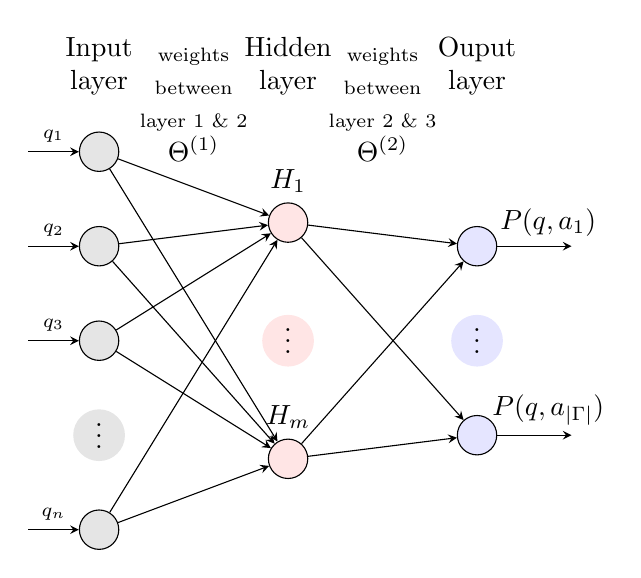
\begin{tikzpicture}[x=1.2cm, y=1.2cm, >=stealth]
\tikzset{%
  every neuron/.style={
    circle,
    draw,
    minimum size=0.5cm
  },
  neuron missing/.style={
    draw=none, 
    scale=1,
    text height=0.333cm,
    execute at begin node=\color{black}$\vdots$
  },
}

\foreach \m/\l [count=\y] in {1,2,3,missing,4}
  \node [fill=black!10,every neuron/.try, neuron \m/.try] (input-\m) at (0,2.5-\y) {};

\foreach \m [count=\y] in {1,missing,2}
  \node [fill=red!10,every neuron/.try, neuron \m/.try ] (hidden-\m) at (2,2-\y*1.25) {};

\foreach \m [count=\y] in {1,missing,2}
  \node [fill=blue!10,every neuron/.try, neuron \m/.try ] (output-\m) at (4,1.5-\y) {};

\foreach \l [count=\i] in {1,2,3,n}
  \draw [<-] (input-\i) -- ++(-0.75,0)
    node [above, midway] {\scriptsize$q_\l$};

\foreach \l [count=\i] in {1,m}
  \node [above] at (hidden-\i.north) {$H_\l$};

\foreach \l [count=\i] in {1,|\Gamma|}
  \draw [->] (output-\i) -- ++(1,0)
    node [above, midway] {\quad $\mathbb{P}(\bm{q}, a_{\l})$};

\foreach \i in {1,...,4}
  \foreach \j in {1,...,2}
    \draw [->] (input-\i) -- (hidden-\j);

\foreach \i in {1,...,2}
  \foreach \j in {1,...,2}
    \draw [->] (hidden-\i) -- (output-\j);

\foreach \l [count=\x from 0] in {Input, Hidden, Ouput}
  \node [align=center, above] at (\x*2,2) {\l \\ layer};
\node[align=center] at (1,2) {\scriptsize weights \\ \scriptsize between \\ \scriptsize layer 1 \& 2 \\ $\bm{\Theta}^{(1)}$};
\node[align=center] at (3,2) {\scriptsize weights \\ \scriptsize between \\ \scriptsize layer 2 \& 3 \\ $\bm{\Theta}^{(2)}$};
\end{tikzpicture}
\caption{A high-level depiction of an artificial NN.}
\label{Fig:FigTwo}
\end{figure}

An artificial NN is simply a set of these logistic units strung together as shown in Figure~\ref{Fig:FigTwo}. Each two layers are connected together using weight parameters. As such, the NN in Figure~\ref{Fig:FigTwo} possesses two weighting matrices, $\bm{\Theta}^{(1)}$ and $\bm{\Theta}^{(2)}$. Here, we used $\bm{\Theta}^{(l)}$ to denote the weights connecting layers $l$ and $l+1$. Definitely, the dimensionality of $\bm{\Theta}^{(l)}$ depends on the number of units in each of the two layers\footnote{
In practice, a bias term is added to increase the expressiveness of the functions learnt by the NN.}. 

For example, in our case, the dimension of the input layer is equal to the number of components, and the dimension of the output layer is equal to number of interactions. The number of hidden layers and the number of neurons per hidden layer can be configured depending on the functions to be learnt. 
%For example, if layer $l$ consists of $s_{l}$ units and layer $l+1$ of $s_{l+1}$, $\bm{\Theta}^{(l)}$ has a dimensionality of $s_{l+1} \times s_{l} +1$, where we have added another dimension to incorporate the bias term (incorporated to increase the expressiveness of the functions learnt by the neural network). 
%

\paragraph{Feed Forward.}
Given the notation introduced above, we are now ready to discuss the computations that are performed by a NN. Intuitively, between every two layers the inputs from the previous layer are, first, linearly (through the weight matrices) propagated forward and then nonlinearly transformed (through the sigmoids) to produce an output on the successor layer. Recursing this process, which we refer to as forward propagation, over the total layers of the network will produce an output on the final layer $L$. 
%

\paragraph{Training \& Backward Propagation.} Having described feed forward propagation, the next step is to detail the strategy by which NNs determine the model parameters (i.e., the $\bm{\Theta}^{(l)}$ matrices -- denoted by $\bm{\Theta}$, i.e., $\bm{\Theta} = \{\bm{\Theta^{(1)}}, \dots, \bm{\Theta^{(L)}}\}$). In standard regression or classification problems, back-propagation is the algorithm adopted. Given an input data point, back-propagation commences as follows. First, forward propagation is executed and the network is made to output a value. This value is then compared to the real output from the data set producing an error. This error is then propagated backwards to every other layer and used to update connecting weights. Such updates typically involve gradient-based methods (e.g., stochastic gradients). 